% Seeded from ../notebooks/lesson_39.ipynb; all nonempty source cells retained.
% The canonical notebook identifies itself as Lessons 39 and 40.
% L39_f24.ipynb instead covers reactor-control perturbation; this handout follows
% the same-number canonical notebook. Local course-color figure renderings
% retain numerical/tracing provenance in figures/drafts/manifest.json.
\documentclass[compact]{ne630handout}
\handoutsolutionsfalse
\begin{document}
\Lesson{39}{Numerical Diffusion and Transport}{\nolinkurl{notebooks/lesson_39.ipynb}.}{Numerical methods to answer questions like \emph{What does the flux look like in two-group problems?} and \emph{When is ``diffusion theory'' a good approximation?}}
\begin{handoutflow}

% Notebook cell 0 (markdown)
\Sec{1}{NE 630 - Lesson 39 and 40...}

\textbf{LAST TIME}: Modeling reactor control (and control "worth").


\textbf{TODAY}:  Numerical methods to answer questions like \emph{What does the flux look like in two-group problems?} and \emph{When is "diffusion theory" a good approximation?}


\textbf{NEXT TIME}: Review \& Practice I

% End notebook cell 0

% Notebook cell 1 (markdown)
\Sec{2}{Review: Perturbation Theory}
% End notebook cell 1

% Notebook cell 2 (markdown)
For a bare slab of width $a$, and given $\phi(x)$, $\nu\Sigma_f(x)$, and $\Sigma_a(x)$, we can write


\begin{equation*}
k = \frac{\text{gains}}{\text{losses}} =
  \frac{\displaystyle \int^{a/2}_{-a/2} \nu\Sigma_f(x) \phi(x) dx}
       {\displaystyle\int^{a/2}_{-a/2} \Sigma_a(x) \phi(x) dx + \text{leakage}} \, .
\tag{1}
\end{equation*}

Now, given a new, slightly perturbed absorption cross section of $\Sigma_a(x) + \delta \Sigma_a$, what's $k$?

% End notebook cell 2

% Notebook cell 3 (markdown)
The naïve approach: just substitute $\Sigma_a = \Sigma_a + \delta \Sigma_a$ into Eq. (1) to get


\begin{equation*}
\delta \rho  \approx
- \frac{ \displaystyle \int_{a/2}^{-a/2}
   \delta\Sigma_a(x) \phi(x) dx}
   { \displaystyle \int_{-a/2}^{a/2}  \nu\Sigma_f(x) \phi(x) dx}\, .
   \tag{2}
\end{equation*}
% End notebook cell 3

% Notebook cell 4 (markdown)
The better approach: weight the integrands by $\phi^*(x)=\phi(x)$:


\begin{equation*}
\delta \rho \approx - \frac{ \displaystyle \int_{-a/2}^{a/2} \phi^*(x)
   \left(\delta\Sigma_a(x)- \frac{\delta \nu\Sigma_f(x)}{k} \right) \phi(x) dx}
   { \displaystyle \int_{-a/2}^{a/2} \phi^*(x) \nu\Sigma_f(x) \phi(x) dx}
\tag{3}
\end{equation*}
% End notebook cell 4

% Notebook cell 5 (markdown)
Quick points on HW 38:


\begin{itemize}

\item HW 38 extended to W @ 11:59pm

\item Check out the extended slides from last time!

\item Is $\int x J_0^2(x) dx$ causing you grief?

\end{itemize}
% End notebook cell 5

% Notebook cell 6 (markdown)
\begin{handoutsmall}[8]
\begin{equation*}
\int x J_0^2(x) = \overbrace{\left [ \frac{x^2 J_0^2}{2} \right ]}^{uv}
  - \overbrace{\int x^2 J_0(x) J_1(x)dx}^{\int vdu} \, \quad \ldots \text{and so on...} = \displaystyle \frac{x^{2} J^{2}_{0}\left(x\right)}{2} + \frac{x^{2} J^{2}_{1}\left(x\right)}{2}
\end{equation*}
\end{handoutsmall}
% End notebook cell 6

% Notebook cell 7 (code)
\begin{NEunicodecode}
import sympy as sy
x = sy.symbols('x')
sy.integrate(x*sy.besselj(0, x)**2)
\end{NEunicodecode}
\begin{equation*}
\displaystyle \frac{x^{2} J^{2}_{0}\left(x\right)}{2} + \frac{x^{2} J^{2}_{1}\left(x\right)}{2}
\end{equation*}
% End notebook cell 7

% Notebook cell 8 (markdown)
\Sec{3}{On Two-Group Diffusion Theory}
% End notebook cell 8

% Notebook cell 9 (markdown)
For HW 37, you used the modified 1-group equation, and without anything else, all we can do is write


\begin{equation*}
\phi_2(x) = \frac{\Sigma_{s_{2\gets 1}} \phi_1(x)}{\Sigma_{a_2}} \, .
\end{equation*}
% End notebook cell 9

% Notebook cell 10 (markdown)
\begin{center}
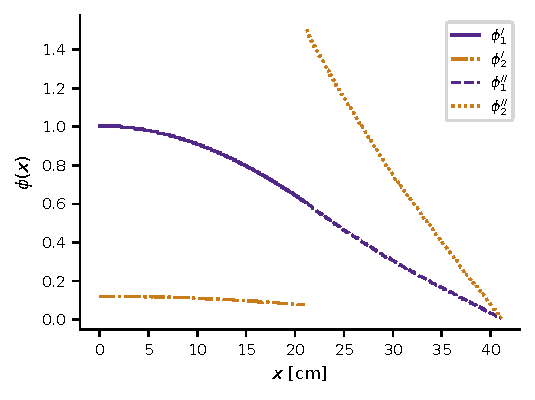
\includegraphics[width=\linewidth,height=.32\textheight,keepaspectratio]{figures/drafts/lesson39_cell10.pdf}
\end{center}
% End notebook cell 10

% Notebook cell 11 (markdown)
\begin{center}
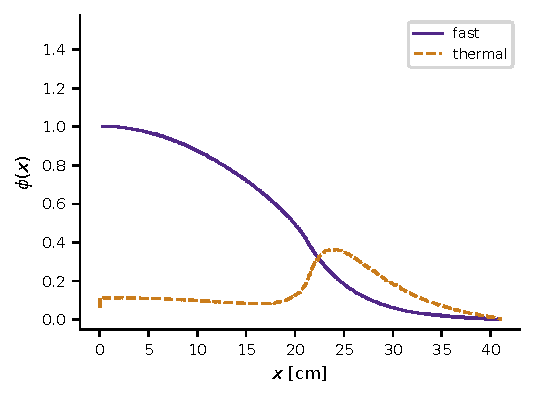
\includegraphics[width=\linewidth,height=.32\textheight,keepaspectratio]{figures/drafts/lesson39_cell11.pdf}
\end{center}
% End notebook cell 11

% Notebook cell 12 (markdown)
\Sec{4}{On the Validity of Diffusion}
% End notebook cell 12

% Notebook cell 13 (markdown)
What was our primary approximation to go from


\begin{equation*}
\vec{\nabla} \cdot \vec{J}(\vec{r})
  + \Sigma_a(\vec{r}) \phi(\vec{r}) = s'''(\vec{r})
  + \nu\Sigma_f(\vec{r}) \phi(\vec{r}) \, ,
  \tag{6.10}
\end{equation*}

to


\begin{equation*}
- \vec{\nabla} \cdot D(\vec{r}) \vec{\nabla} \phi(\vec{r})
  + \Sigma_a(\vec{r}) \phi(\vec{r}) = s'''(\vec{r})
  + \nu\Sigma_f(\vec{r}) \phi(\vec{r}) \, ?
  \tag{6.12}
\end{equation*}
% End notebook cell 13

% Notebook cell 14 (markdown)
Answer: Fick's law, i.e., $\vec{J} \approx -D(\vec{r})\vec{\nabla}\phi(\vec{r})$

% End notebook cell 14

% Notebook cell 15 (markdown)
\Sec{5}{Review Problem}

Consider a slab of width 20 cm with $\Sigma_t = 1$ cm and $\Sigma_a = 0.01$ cm with a uniform source of strength $s'''=1$ [1/cm$^3$-s] subject to vacuum.  Find $\phi(x)$.

% End notebook cell 15

% Notebook cell 16 (markdown)
Last time, we started with


\begin{equation*}
- \phi''(x) + \frac{1}{L^2}\phi(x) = \frac{s'''}{D} \,
\end{equation*}

and found that


\begin{equation*}
\phi(x) = \overbrace{C_1 \cosh(x/L) + C_2 \sinh(x/L)}^{\phi_h}
          + \overbrace{\frac{L^2 s'''}{D}}^{\phi_p} \, ,
\end{equation*}

where $L^2 = D/\Sigma_a$, subject to $\phi(a/2) = \phi(-a/2) = 0$ (i.e., simple zero-flux conditions).

% End notebook cell 16

% Notebook cell 17 (markdown)
Our right BC is


\begin{equation*}
\phi(a/2) = 0 = C_1 \cosh(a/2L) + C_2 \sinh(a/2L) + \frac{L^2 s'''}{D}
\end{equation*}

and our left BC is


\begin{equation*}
\begin{split}
  \phi(-a/2) = 0 &= C_1 \cosh(-a/2L) + C_2 \sinh(-a/2L) + \frac{L^2 s'''}{D}  \\
             &= C_1 \cosh(a/2L) - C_2 \sinh(a/2L) + \frac{L^2 s'''}{D}
\end{split}
\end{equation*}
% End notebook cell 17

% Notebook cell 18 (markdown)
Subtract the left BC from the right BC to find


\begin{equation*}
2C_2 \sinh(a/2L) = 0 \quad \longrightarrow \quad C_2 = 0 \, .
\end{equation*}

Then


\begin{equation*}
C_1 \cosh(a/2L) = \frac{L^2 s'''}{D} \quad \longrightarrow \quad C_1 = -\frac{L^2 s'''}{D\cosh(a/2L)} \, ,
\end{equation*}

and


\begin{equation*}
\phi(x) = -\frac{L^2 s''' \cosh(x/L)}{D\cosh(a/2L)} + \frac{L^2 s'''}{D} = \boxed{ \frac{s'''}{\Sigma_a} \left (1 - \frac{\cosh(x/L)}{\cosh(a/2L)} \right )} \, .
\end{equation*}
% End notebook cell 18

% Notebook cell 19 (code)
\begin{NEunicodecode}
import numpy as np
import matplotlib.pyplot as plt
plt.rcParams['figure.figsize'] = [12, 6]
plt.rcParams['figure.dpi'] = 100 # 200 e.g. is really fine, but slower

plt.rcParams['font.family'] = 'Serif'
plt.rcParams["mathtext.fontset"] = "dejavuserif"
plt.rcParams['font.size'] =  22
plt.rcParams['lines.linewidth'] = 2
s = 1; D = 1/3; Sigma_a = 0.01; a = 20; L = np.sqrt(D/Sigma_a)
x = np.linspace(-a/2, a/2, 1000)
phi = (s/Sigma_a)*(1-np.cosh(x/L)/np.cosh(a/2/L))

plt.plot(x, phi); plt.xlabel('$x$'); plt.ylabel("$\phi(x)$");
\end{NEunicodecode}
\begin{center}
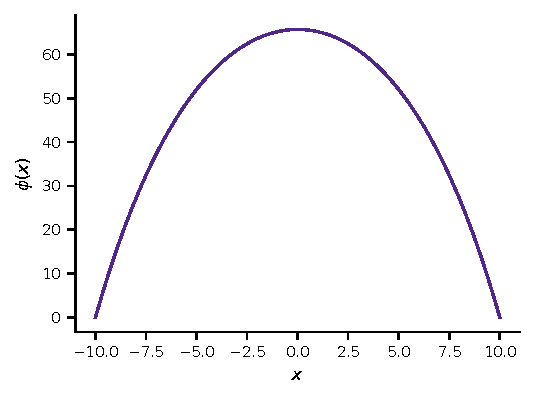
\includegraphics[width=\linewidth,height=.32\textheight,keepaspectratio]{figures/drafts/lesson39_cell19.pdf}
\end{center}
% End notebook cell 19

% Notebook cell 20 (markdown)
Now, how does this compare to the diffusion solution with vacuum? With the \emph{neutron transport} solution?

% End notebook cell 20

% Notebook cell 21 (code)
\begin{NEunicodecode}
import sys
sys.path.append("/home/robertsj/Research/detran/pydetran/build")

import detran
from detran import InputDB, Material, Fixed1D, Mesh1D, IsotropicSource

def get_input():
    """ fills default input parameters.
    """
    # Input
    inp = InputDB()
    inp.put_str("problem_type",       "fixed")
    inp.put_int("number_groups",      1)
    inp.put_str("equation",           "diffusion")
    inp.put_str("inner_solver",       "SI")
    inp.put_int("inner_max_iters",    10000)
    inp.put_dbl("inner_tolerance",    1e-12)
    inp.put_int("inner_print_level",  1)
    inp.put_int("outer_max_iters",    10000)
    inp.put_dbl("outer_tolerance",    1e-8)
    inp.put_int("outer_print_level",  1)
    inp.put_str("quad_type",                  "gl")
    inp.put_int("quad_number_polar_octant",   32)
    inp.put_str("bc_west",                    "vacuum")
    inp.put_str("bc_east",                    "vacuum")
    db = InputDB("callow_db")
    db.put_dbl("linear_solver_atol",                  1e-12);
    db.put_dbl("linear_solver_rtol",                  1e-12);
    db.put_str("linear_solver_type",                  "gmres");
    db.put_int("linear_solver_maxit",                 5000);
    db.put_int("linear_solver_gmres_restart",         30);
    db.put_int("linear_solver_monitor_level",         0);
    db.put_str("pc_type", "ilut")
    db.put_int("ilu_levels", 1)
    db.put_dbl("ilu_thresh", 0)
    inp.put_spdb("inner_solver_db", db)
    inp.put_spdb("outer_solver_db", db)
    return inp

def get_material():
    mat = Material(4, 1)
    # original material - highly scattering
    mat.set_sigma_t(0, 0, 1.0)
    mat.set_sigma_s(0, 0, 0, 0.99)
    mat.set_diff_coef(0, 0, 1/3.0)
    # same total cross section (and, hence, D) but higher sigma_a
    mat.set_sigma_t(1, 0, 1.0)
    mat.set_sigma_s(1, 0, 0, 0.5)
    mat.set_diff_coef(1, 0, 1/3.0)
    # large cross section with pure absorption
    mat.set_sigma_t(2, 0, 5.0)
    mat.set_sigma_s(2, 0, 0, 0.0)
    mat.set_diff_coef(2, 0, 1/15.0)
    # cross section with sigma_s > sigma_t; numerically equivalent to k_oo>1
    mat.set_sigma_t(3, 0, 1.0)
    mat.set_sigma_s(3, 0, 0, 1.2)
    mat.set_diff_coef(3, 0, 1/3.0)
    #
    mat.compute_sigma_a()
    mat.finalize()
    return mat

def get_mesh(material_map, source_map):
    # break our 20 cm into 20 regions
    cm = np.linspace(0, 20, 21)
    fm = [100]*20
    mesh = Mesh1D(fm, cm, material_map)
    mesh.add_coarse_mesh_map("SOURCE", source_map)
    return mesh

def solve(material_map, source_map, equation, bcL="vacuum", bcR="vacuum"):
    inp = get_input()
    inp.put_str("equation", equation)
    inp.put_str("bc_east", bcR)
    inp.put_str("bc_west", bcL)
    mat = get_material()
    mesh = get_mesh(material_map, source_map)
    solver = Fixed1D(inp, mat, mesh)
    solver.setup()
    source_fm_map = detran.vec_int(mesh.mesh_map("SOURCE"))
    # [#spec][#group].  here, we've got one group, and
    #  so [0.0] is the no-source, and [1.0] is the unit source.
    spectra = detran.vec2_dbl([[0.0], [1.0]])
    q_e = IsotropicSource(1, mesh, spectra, source_fm_map)
    solver.set_source(q_e)
    solver.set_solver()
    solver.solve()
    x = np.linspace(-10, 10, mesh.number_cells()+1)
    x = x[1:]-(x[1]-x[0])/2
    return np.array(solver.state().phi(0)), x
\end{NEunicodecode}
% End notebook cell 21

% Notebook cell 22 (code)
\begin{NEunicodecode}
source_map = [1]*20
material_map = [0]*20
phi_diff, x_vals = solve(material_map, source_map, "diffusion")
phi_tran, x_vals = solve(material_map, source_map, "dd")


plt.plot(x, phi, 'g', label="diffusion: zero flux")
plt.plot(x_vals, phi_diff, 'k', label="diffusion: vacuum")
plt.plot(x_vals, phi_tran, 'b:', label="transport")

plt.xlabel('$x$'); plt.ylabel("$\phi(x)$");
plt.legend();
\end{NEunicodecode}
\begin{NEunicodecode}
    SI Final: Number Iters: 1629  Error:  0.000000000  Sweeps:   1629
  GS Final: Number Iters:   0  Error:  0.000000000  Sweeps:   1629
PCILUT...construction complete.
    Starting SI.
      group 0
\end{NEunicodecode}
\begin{center}
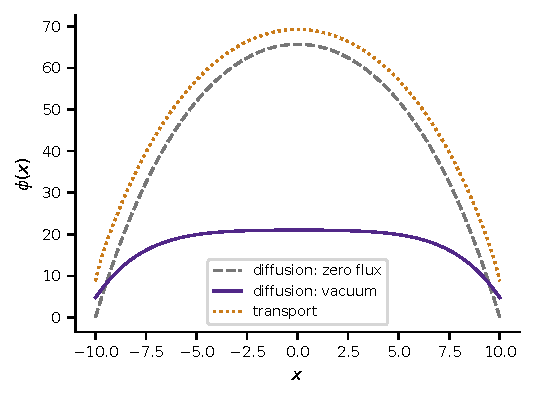
\includegraphics[width=\linewidth,height=.32\textheight,keepaspectratio]{figures/drafts/lesson39_cell22.pdf}
\end{center}
% End notebook cell 22

% Notebook cell 23 (markdown)
Now, omit the zero-flux solution:

% End notebook cell 23

% Notebook cell 24 (code)
\begin{NEunicodecode}
plt.plot(x_vals, phi_diff, 'k')
plt.plot(x_vals, phi_tran, 'b:')
plt.xlabel('$x$'); plt.ylabel("$\phi(x)$");
plt.legend(["diffusion: vacuum", "transport"]);
\end{NEunicodecode}
\begin{center}
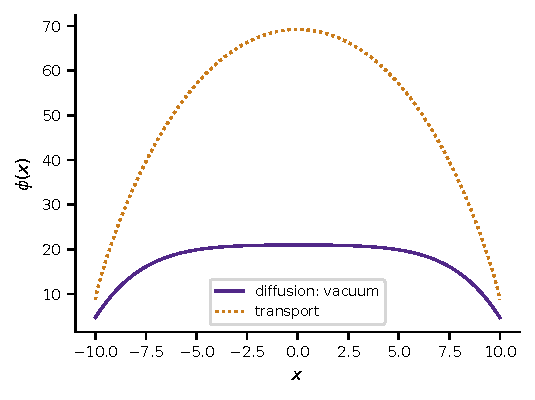
\includegraphics[width=\linewidth,height=.32\textheight,keepaspectratio]{figures/drafts/lesson39_cell24.pdf}
\end{center}
% End notebook cell 24

% Notebook cell 25 (code)
\begin{NEunicodecode}
plt.plot(x_vals, 100*(phi_diff-phi_tran)/phi_tran, "k-")
plt.xlabel('$x$'); plt.ylabel("error (%)");
plt.title("Observation 1: Diffusion Fails at Vacuum Boundaries");
\end{NEunicodecode}
\begin{center}
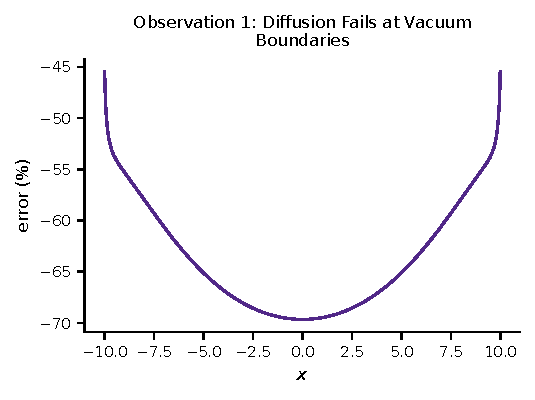
\includegraphics[width=\linewidth,height=.32\textheight,keepaspectratio]{figures/drafts/lesson39_cell25.pdf}
\end{center}
% End notebook cell 25

% Notebook cell 26 (markdown)
\Sec{6}{Example 2: Localized Source with Reflecting Conditions}
% End notebook cell 26

% Notebook cell 27 (code)
\begin{NEunicodecode}
 
material_map = [0]*20
phi_diff, x_vals = solve(material_map, source_map, "diffusion", "reflect", "reflect")
phi_tran, x_vals = solve(material_map, source_map, "dd", "reflect", "reflect")

plt.plot(x_vals, phi_diff, 'k')
plt.plot(x_vals, phi_tran, 'b:')
plt.xlabel('$x$'); plt.ylabel("$\phi(x)$");
plt.legend(["diffusion", "transport"]);
\end{NEunicodecode}
\begin{NEunicodecode}
    SI Final: Number Iters: 2495  Error:  0.000000000  Sweeps:   2495
  GS Final: Number Iters:   0  Error:  0.000000000  Sweeps:   2495
PCILUT...construction complete.
    Starting SI.
      group 0
\end{NEunicodecode}
\begin{center}
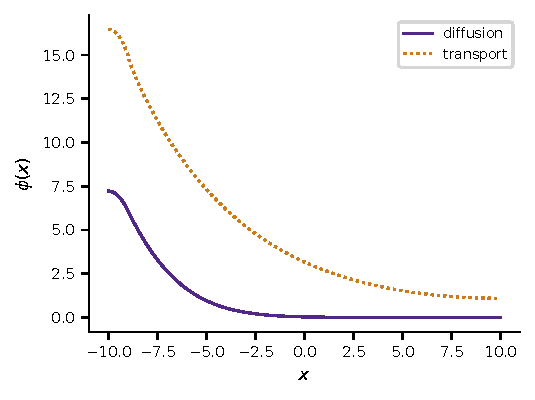
\includegraphics[width=\linewidth,height=.32\textheight,keepaspectratio]{figures/drafts/lesson39_cell27.pdf}
\end{center}
% End notebook cell 27

% Notebook cell 28 (code)
\begin{NEunicodecode}
plt.plot(x_vals, 100*(phi_diff-phi_tran)/phi_tran, "k-")
plt.xlabel('$x$'); plt.ylabel("error (%)");
plt.title("Observation 2: Diffusion Fails near Localized Sources");
\end{NEunicodecode}
\begin{center}
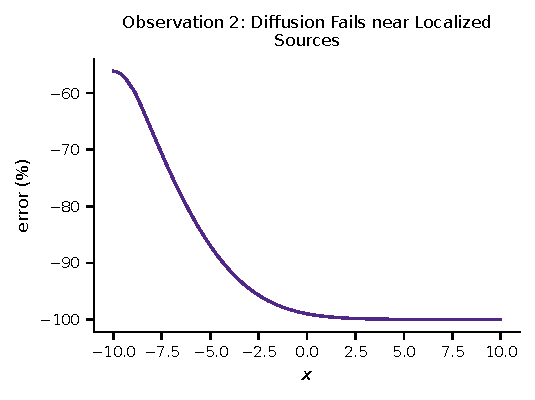
\includegraphics[width=\linewidth,height=.32\textheight,keepaspectratio]{figures/drafts/lesson39_cell28.pdf}
\end{center}
% End notebook cell 28

% Notebook cell 29 (markdown)
\Sec{7}{Example 3: Localized Absorber with Uniform Source and Reflecting Conditions}
% End notebook cell 29

% Notebook cell 30 (code)
\begin{NEunicodecode}
source_map = [1]*20
material_map = [0]*20
material_map[9] = 1
phi_diff, x_vals = solve(material_map, source_map, "diffusion", "reflect", "reflect")
phi_tran, x_vals = solve(material_map, source_map, "dd", "reflect", "reflect")

plt.plot(x_vals, phi_diff, 'k')
plt.plot(x_vals, phi_tran, 'b')
plt.xlabel('$x$'); plt.ylabel("$\phi(x)$");
plt.legend(["diffusion", "transport"]);
\end{NEunicodecode}
\begin{NEunicodecode}
    SI Final: Number Iters: 2495  Error:  0.000000000  Sweeps:   2495
  GS Final: Number Iters:   0  Error:  0.000000000  Sweeps:   2495
PCILUT...construction complete.
    Starting SI.
      group 0
\end{NEunicodecode}
\begin{center}
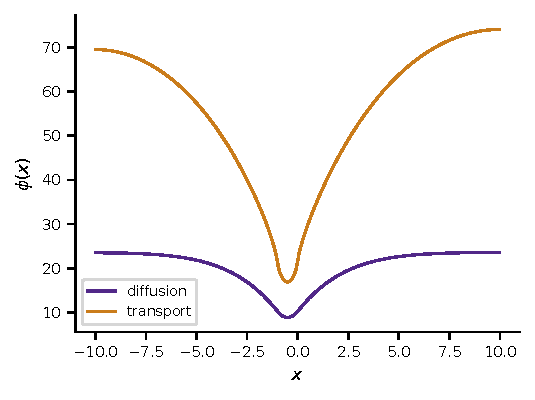
\includegraphics[width=\linewidth,height=.32\textheight,keepaspectratio]{figures/drafts/lesson39_cell30.pdf}
\end{center}
% End notebook cell 30

% Notebook cell 31 (code)
\begin{NEunicodecode}
plt.plot(x_vals, 100*(phi_diff-phi_tran)/phi_tran, 'k-')
plt.xlabel('$x$'); plt.ylabel("error (%)");
plt.title("Observation 3: Diffusion Fails near Localized Absorbers");
\end{NEunicodecode}
\begin{center}
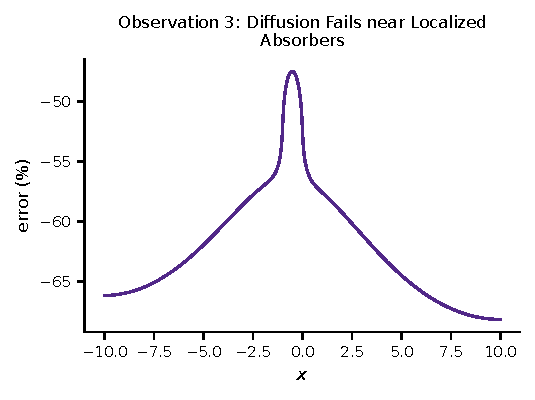
\includegraphics[width=\linewidth,height=.32\textheight,keepaspectratio]{figures/drafts/lesson39_cell31.pdf}
\end{center}
% End notebook cell 31

% Notebook cell 32 (markdown)
\Sec{8}{Summary of Observations}

Predictions from diffusion theory deviate from the more rigorous transport theory near


\begin{enumerate}

\item vacuum conditions

\item localized sources

\item localized (changes in) absorption

\end{enumerate}
% End notebook cell 32

% Notebook cell 33 (markdown)
So, what the heck is \emph{transport theory} doing different?

% End notebook cell 33

% Notebook cell 34 (markdown)
First, a new unknown.  Assume have both a spatial location $\vec{r}$ and a direction $\hat{\Omega} = (\theta, \varphi)$ but all have the same energy (and speed).  Then the neutron density is written $n(\vec{r}, \hat{\Omega})$ and


\begin{equation*}
\psi(\vec{r}, \hat{\Omega}) = v n(\vec{r}, \hat{\Omega}) = \text{angular flux} \, .
\end{equation*}
% End notebook cell 34

% Notebook cell 35 (markdown)
Of course, $\psi(\vec{r}, \hat{\Omega})$ is new to use, but it's closely related to two quantities we've seen a lot:


\begin{equation*}
\phi(\vec{r}) = \int_{4\pi}  \psi(\vec{r}, \hat{\Omega}) d\Omega  = \text{flux}\,
\end{equation*}

\begin{equation*}
\vec{J}(\vec{r}) = \int_{4\pi} \hat{\Omega} \psi(\vec{r}, \hat{\Omega}) d\Omega = \text{current} \,
\end{equation*}
% End notebook cell 35

% Notebook cell 36 (markdown)
In slab geometry, $\hat{\Omega}$ reduces to $\theta$ (the angle of travel relative to the positive $x$ axis), and with $\mu = \cos{\theta}$, we have


\begin{equation*}
\phi(x) = \int^{1}_{-1} \psi(x, \mu) d\mu \qquad \text{and} \qquad J(x) = \int^{1}_{-1} \mu \psi(x, \mu) d\mu \, .
\end{equation*}
% End notebook cell 36

% Notebook cell 37 (markdown)
The equation that governs $\psi(x, \mu)$ is the \emph{transport equation}.  If scattering is isotropic in the lab system (i.e., the average scattering cosine is $\bar{\mu}_0 = 0$), we have


\begin{equation*}
\mu \frac{\partial \psi}{\partial x} + \Sigma_t \psi(x, \mu) = \frac{\Sigma_s}{2} \phi(x) + \frac{s'''(x)}{2} \, ,
  \tag{1}
\end{equation*}

subject to


\begin{equation*}
\psi(x_L, \mu) = \psi_L, \, \mu > 0 \qquad \text{and} \qquad \psi(x_R, \mu) = \psi_R, \, \mu < 0 \, .
\end{equation*}

Here, $\psi_L = \psi_R = 0$ represents a true vacuum condition.

% End notebook cell 37

% Notebook cell 38 (markdown)
Treating $\mu$ is an important part of solving problems in transport theory.  Let's keep our life simple and guess that


\begin{equation*}
\begin{aligned}
\psi(x, \mu) = \psi_0(x) + \mu \psi_1(x) \qquad \longrightarrow \\ \qquad \phi(x) = 2\psi_0(x) \quad \text{and} \quad J(x) = \frac{3}{2}\psi_1(x) \, .
\end{aligned}
\end{equation*}

Plugging this into the NTE leads to


\begin{equation*}
\displaystyle \mu \frac{d}{d x} \psi_{0}{\left(x \right)} +  \mu^{2} \frac{d}{d x} \psi_{1}{\left(x \right)}  + \Sigma_{t} ( \psi_{0}{\left(x \right)} + \mu \psi_{1}{\left(x \right)} ) = \Sigma_{s} \psi_{0}{\left(x \right)} + \frac{s'''{\left(x \right)}}{2} \, .
  \tag{2}
\end{equation*}
% End notebook cell 38

% Notebook cell 39 (markdown)
Now, integrate Eq. (2) over $\mu$ to get


\begin{equation*}
\frac{2}{3}\frac{d \psi_1}{dx} + 2\Sigma_t \psi_0(x) = 2\Sigma_s \psi_0(x) + s'''(x) \, .
  \tag{3}
\end{equation*}
% End notebook cell 39

% Notebook cell 40 (markdown)
Similarly, multiply Eq. (2) by $\mu$ and integrate again to get


\begin{equation*}
\frac{2}{3} \frac{d\psi_0}{dx} = -\frac{2\Sigma_t}{3} \psi_1(x) \, .
  \tag{4}
\end{equation*}
% End notebook cell 40

% Notebook cell 41 (markdown)
From (4), we have


\begin{equation*}
\psi_1(x) = -\frac{1}{\Sigma_t} \frac{d\psi_0}{dx} \longrightarrow \boxed{J(x)
    = -\frac{1}{3\Sigma_t} \frac{d\phi}{dx} = -D \frac{d\phi}{dx} } \, ,
  \tag{5}
\end{equation*}

and substituting this into Eq. (3) and moving scattering to the left, we have


\begin{equation*}
-\frac{2}{3\Sigma_t}\frac{d^2\psi_0}{dx^2} + 2(\Sigma_t-\Sigma_s)\psi_0(x) = s'''(x)
  \longrightarrow \boxed{-D\phi'' + \Sigma_a \phi(x) = s'''(x)} \, .
  \tag{6}
\end{equation*}
% End notebook cell 41

% Notebook cell 42 (markdown)
In summary, diffusion theory is equivalent to assuming that the distribution of neutron directions with respect to each Cartesian axis is linear.   Things like vacuum boundaries (that's a \emph{step} function in angle!), strong absorbers (that's exponential attenuations!), and localized sources (that's again like a \emph{step} function) all break that assumption to varying degrees!

% End notebook cell 42

% Notebook cell 43 (code)
% Empty source cell.
% End notebook cell 43

\end{handoutflow}
\end{document}
